% select subfiles base file
\documentclass[TGAI_Laborbericht.tex]{subfiles}
\begin{document}

\chapter{Versuch 4}
\label{chap:VERSUCH_4}

\section{Fragestellung, Messprinzip, Aufbau, Messmittel}
\label{chap:VERSUCH_4_FRAGESTELLUNG}
Wir sollen nun das Dunkelbild auf hot und stuck pixel sowie das Weißbild auf dead pixel untersuchen und diese auf den bildern kenntlich machen. Außerdem wird nun das ursprüngliche Graukeil Bild mithilfe des Dunkel und Weißbildes korrigiert. Anschließend werden die Mittelwerte und Standartabweichungen des ursprünglichen Bildes und des korrigierten Bildes gegenübergestellt.

\section{Messwerte}
\label{chap:VERSUCH_4_MESSWERTE}
\begin{figure}[H]
	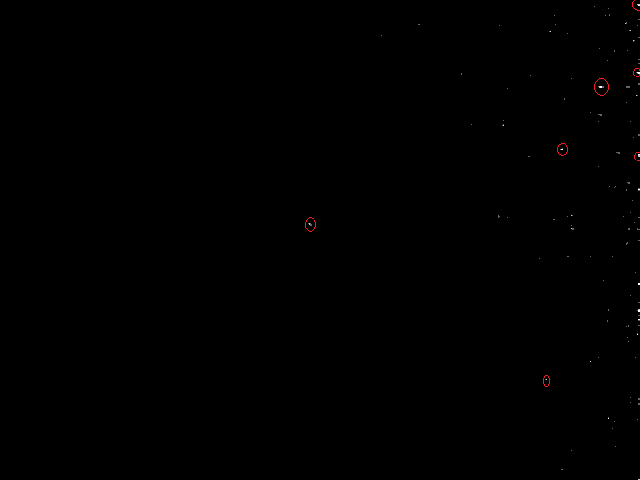
\includegraphics[width=0.7\textwidth]{media/stuck&hotpixel.png}
	\caption{stuck und hot pixel}
	\label{fig:stuck und hot pixel}
\end{figure}

\section{Auswertung}
\label{chap:VERSUCH_4_AUSWERTUNG}

\section{Interpretation}
\label{chap:VERSUCH_4_INTERPRETATION}

\end{document}